% Chapter 3

\chapter{Case Study} % Main chapter title

\label{Chapter2} % For referencing the chapter elsewhere, use \ref{Chapter1} 

\lhead{Chapter 2. \emph{Case Studies}} % This is for the header on each page - perhaps a shortened title

%----------------------------------------------------------------------------------------

\section{General Design Considerations of Senior Population}
There are several main categories of housing choices for the elderly:
independent living communities, assisted living, Continuing Care
Retirement Communities (CCRC), nursing homes, and alzheimer's care.

The senior community center under discussion in the current project
aims at providing diverse choices for degree of assist, hence it is
not easy to categorize it into one of the categories above. It also
integrates with the university population, making the function even
further from a traditional senior center setting. The case study in
this section focus more on the aspect specific to the project, such as
the affiliation to a university, and a combined facility of living and
research.

\section{Elderly and Children Combined Facility}
\subsection{Altersheim Furttal, A Retirement Home in a Swiss Village}
The retirement home is built near the city center with good public
transportation. This connection provides the residents with a stronger
connection to the society.

There is a kindergarten to the north of the facility. The connections
between the two age groups are established with a common courtyard
between the kindergarten and the retirement home. The interior space
design strengthens this connection by arranging a two story ``lounge
space'' adjacent to the common garden.

\begin{figure}
\centering
\begin{subfigure}{0.7\textwidth}
  \centering
  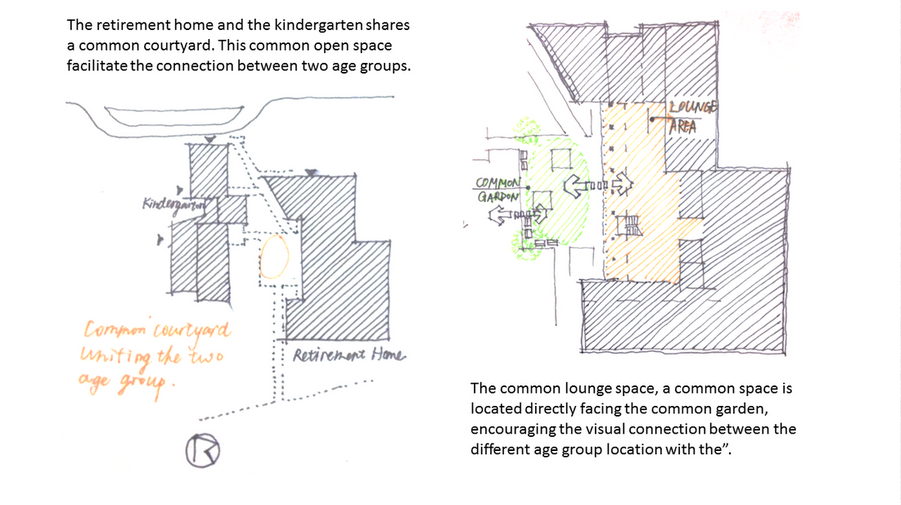
\includegraphics[width=\linewidth]{case1.png}
  \caption{Site Plan Layout of Altersheim Furttal and Kindergarten}
  \label{fig:case1}
\end{subfigure}
\begin{subfigure}{0.7\textwidth}
  \centering
  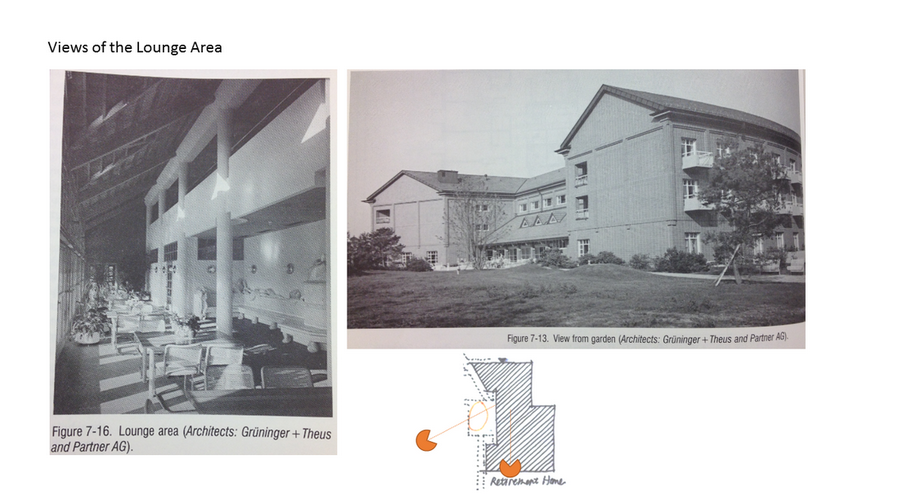
\includegraphics[width=\linewidth]{case2.png}
  \caption{Views of the Lounge Area}
  \label{fig:case2}
\end{subfigure}
\caption{Common Garden and Interior Design in Creating Connections
  between Different Age Groups}
\label{fig:case2}
\end{figure}
\section{University Affiliated Senior Housing}
\section{Dementia Assisted Living}
``Dementia is an umbrella term for a group of cognitive disorders
typically characterized by memory impairment, as well as marked
difficulty in the domains of language, motor activity, object
recognition, and disturbance of executive function – the ability to
plan, organize, and abstract.''~\cite{CDCdementia} Dementia, or its
most common form Alzheimer is highly prone and one could not neglect
its existance: there are 5 million Alzheimer victims in the U.S. and
every 1 out of 3 seniors die in dementia. Women are more vulnerable to
dementia and 2/3 of the Alzheimer victims are
women~\cite{alzorg2014}. This section conduct some related case study
on elderly caring facilities for people with Alzheimer Diseases. 

The physical space acted as a ``therapeutic resource'' in improving
the wellbeing and help reduce the seriousness of
dementia~\cite{Day2000}. Relocation of individual dementia victims to
new environments can increase the possibility of depression and
mortality~\cite{ANTHONY01111987}. This implies the necessity for
dementia dedicated space. If there are not such spaces, when resident
develops dementia, they will have to be relocated to facilities that
has dementia care functions, which might cast negative impact. The
living unit for cognitively impared people are commonly refered to as
Spetial Care Unit (SCU). The common features of SCUs include ``smaller
size units, fewer resident rooms and more designated private rooms
with private dining rooms''. The SCU environment have positive impact
on ``communication, self-care, social function and mobility'' status
of dementia victims. It also reduce emotional strain and increase
satisfactions. Separation between people with and without dementia is
necessary as study showed non-dementia residents experience mental
declines as a result of living near dementia victims. The tipical
features of a SCU unit include: less rooms, small room sizes, private
rooms and dining space, access to outdoor environment
etc~\cite{Day2000}. Smaller cluster size showed positive effects on
reducing agitation level, aggressiveness, anxiety and
depression~\cite{Day2000}. The positive impact of smaller cluster
group setting also includes relief of stress and negative attitude of
relative care-givers~\cite{Annerstedt19931529, Day2000}. Special
acoustic feature should be added to create a balance between ``sensory
overstimulation'' and ``deprivation'', i.e. create a space that is
neither too noisy nor too quiet. Since people with dimentia tend to
also have visual difficulties, the suggested visual environment is low
glare, high contrast and increase lighting level~\cite{Day2000}. The
``bright light treatment'' showed improvement on sleep
patterns~\cite{Mishima1994}. For enhancing way-finding, common design
suggestions include: provide views to the outside environment which
gives hint of location; create ``landmarks'', large signs; increase
lighting level of public spaces etc. Corridors are associated with
less orientation and higher percentage of hallway reduces
disorientation~\cite{Day2000}
\section{Sustainable Strategy in Senior Center}